\apendice{Especificación de diseño}

\section{Introducción}
En este anexo se explican los diseños que se han llevado a cabo para realizar los objetivos anteriores al igual que se describen los usados utilizados para conseguirlo.

\section{Diccionario de datos}

\subsection{Summoners}
\textit{Summoners} (tabla~\ref{tabla:jugador}) representa a la entidad del jugador.
\tablaSmall{Entidad del jugador}{lXl}{jugador}{Variable & Descripción & Tipo \\}
{
accountId & Identificador de la cuenta a nivel de región & String \\
name & Nombre del jugador dentro del juego & String \\
region & Identificador de la región & String \\
puuid & Identificador global de la cuenta & String \\
summonerId & Identificador del jugador a nivel de región & String \\
}

\subsection{Matches}
\textit{Matches} (tabla~\ref{tabla:partida}) es la entidad referida a las partidas jugadas. Se muestran solo los atributos relevantes para este problema ya el bruto contiene demasiada información que no aporta valor a este problema.
\tablaSmall{Entidad de la partida}{lXl}{partida}{Variable & Descripción & Tipo \\}
{
creation & Fecha y hora en la que comienza la partida & Timestamp \\
region & Identificador de la región & String \\
version & Identificador de la versión del juego en la que se ha jugado la partida & String \\
gameId & Identificador de la partida & Integer \\
teams & Lista que contiene a los dos equipos, siempre tiene tamaño dos & Array \\
teams.participants & Lista que contiene a los jugadores del equipo, siempre tiene tamaño cinco & Array \\
teams.participants.stats & Varias estadísticas del jugador al terminar la partida & Map \\
teams.participants.stats.item0 & Identificador del primer objeto & Integer \\
teams.participants.stats.item1 & Identificador del segundo objeto & Integer \\
teams.participants.stats.item2 & Identificador del tercer objeto & Integer \\
teams.participants.stats.item3 & Identificador del cuarto objeto & Integer \\
teams.participants.stats.item4 & Identificador del quinto objeto & Integer \\
teams.participants.stats.item5 & Identificador del sexto objeto & Integer \\
teams.participants.championId & Identificador del campeón seleccionado por el jugador & Integer \\
teams.participants.position & Posición en la que se ha jugador el campeón seleccionado por el jugador & String \\
}

\subsection{Transactions}
\textit{Transactions} (tabla~\ref{tabla:transacciones}) es la entidad que representa los datos de entrada que se van a suministrar al algoritmo Apriori. Es el resultado de la fase de transformación de la \textit{pipeline}.
\tablaSmall{Transacciones}{lXl}{transacciones}{Variable & Descripción & Tipo \\}
{
champion & Identificador del jugador & Integer \\
position & Posición en la que se ha jugado al campeón & String \\
transactions & Listado de conjuntos de objetos que ha tenido el campeón en la posición & Array<Array> \\
transactions.* & Conjunto de objetos con los que el campeón ha terminado la partida & Array<Integer> \\
}

\subsection{Frequent builds}
\textit{Frequent builds} (tabla~\ref{tabla:frequent-builds}) son los datos que se muestran en la aplicación web al usuario final. Contienen la salida del algoritmo Apriori y atributos para identificar al campeón y posición.
\tablaSmall{Conjuntos frecuentes de objetos}{lXl}{frequent-builds}{Variable & Descripción & Tipo \\}
{
champion & Identificador del jugador & Integer \\
games & Cantidad de partidas jugadas con el campeón llevado en una posición & Integer \\
position & Posición en la que se ha jugado al campeón & String \\
builds & Listado de conjuntos frecuentes de objetos & Array \\
builds.support & Porcentaje de veces que aparece el conjunto de objetos en el listado de transacciones & Float \\
builds.itemset & Conjunto de objetos frecuentes encontrado por el algoritmo & Array \\
}


\section{Diseño procedimental}
En esta sección se incluirán varios diagramas para comprender mejor cada una de las fases por las que se ha pasado hasta conseguir los conjuntos frecuentes que se van a mostrar al usuario.

\subsection{Extracción de jugadores}
La primera fase es la extracción de jugadores, se obtienen desde la API, se añade el identificador de cuenta y se guardan.
\begin{figure}[h]
	\centering
	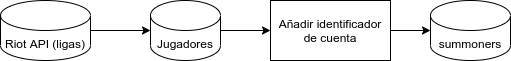
\includegraphics[width=1\linewidth]{img/diag-summoners}
	\caption{Extracción de jugadores}
	\label{fig:diag-summoners}
\end{figure}

\subsection{Extracción de partidas}
A continuación se obtienen las partidas de cada jugador, se añade la posición y se guardan.
\begin{figure}[h]
	\centering
	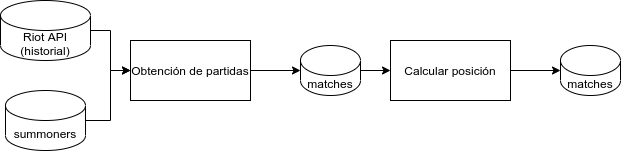
\includegraphics[width=1\linewidth]{img/diag-matches}
	\caption{Extracción de partidas}
	\label{fig:diag-matches}
\end{figure}

\subsection{Generación de transacciones y conjuntos frecuentes}
A partir de las partidas, se ejecuta la agregación en MongoDB y se guardan. A continuación se usan las transacciones como entrada para el Apriori y se guarda la salida en la colección final.
\begin{figure}[h]
	\centering
	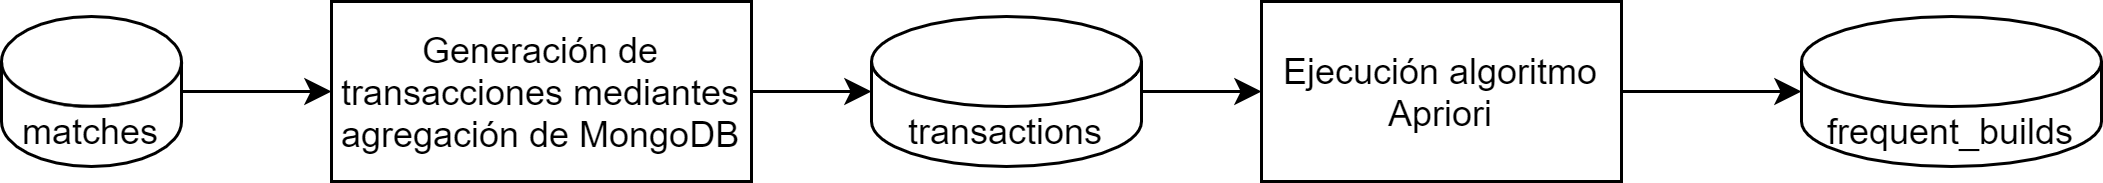
\includegraphics[width=1\linewidth]{img/diag-transform}
	\caption{Generación de transacciones y conjuntos frecuentes}
	\label{fig:diag-matches}
\end{figure}